Veeam läuft auf einem Windows Server 2016 mit einer Topologie,
ersichtlich in Abbildung \ref{veeam-grob}.

\begin{figure}[!htb]
\centering
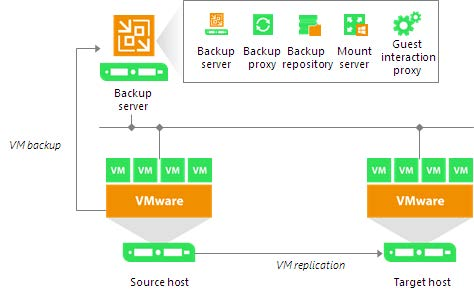
\includegraphics{./images/veeam_grob.jpg}
\caption{Veeam Aufbau}\label{veeam-grob}
\end{figure}

\hypertarget{installation}{%
\section{Installation}\label{installation}}

\begin{enumerate}
\def\labelenumi{\arabic{enumi}.}
\item
  Software von Veeam herunterladen von der
  \href{www.veeam.com/downloads.html}{Veeam Download Seite}
\item
  Software als ISO in eine VM einlegen
\item
  Setup.exe in der VM ausführen und im Wizard auf Install clicken
\item
  Lizenzeinstellungen akzeptieren und ohne Lizenzdatei fortfahren
\item
  Veeam Backup \& Replication sowie die zugehörige Console im Wizard
  auswählen
\item
  fehlende Software automatisch nachinstallieren lassen
\item
  Installationsdetails auswählen

  \begin{longtable}[]{@{}ll@{}}
  \toprule
  Einstellung & Wert\tabularnewline
  \midrule
  \endhead
  Installationsordner & C:\textbackslash Program
  Files\textbackslash Veeam\textbackslash Backup and
  Replication\tabularnewline
  vPower Cache &
  C:\textbackslash ProgramData\textbackslash Veeam\textbackslash Backup\textbackslash NfsDatastore\tabularnewline
  Guest Catalog & C:\textbackslash VBRCatalog\tabularnewline
  Catalog Service Port & 9393\tabularnewline
  Service Port & 9392\tabularnewline
  Secure Connections Port & 9401\tabularnewline
  Service Account & LOCAL SYSTEM\tabularnewline
  SQL Server & LOCALHOST\textbackslash VEEAMSQL2012\tabularnewline
  Datenbank Name & VeeamBackup\tabularnewline
  \bottomrule
  \end{longtable}
\item
  Installation abschließen
\end{enumerate}

\hypertarget{hinzufuxfcgen-des-hypervisors}{%
\section{Hinzufügen des
Hypervisors}\label{hinzufuxfcgen-des-hypervisors}}

\begin{enumerate}
\def\labelenumi{\arabic{enumi}.}
\tightlist
\item
  Veeam Dienste starten
\item
  Veeam Backup and Replication Console öffnen
\item
  Neuen VMware Server Wizard starten

  \begin{enumerate}
  \def\labelenumii{\arabic{enumii}.}
  \tightlist
  \item
    Backup Infrastruktur öffnen
  \item
    im Tab Verwaltete Server neuen Server hinzufügen
  \item
    VMware Vsphere auswählen
  \item
    Server-Details eintragen
  \end{enumerate}
\item
  Überprüfung

  \begin{enumerate}
  \def\labelenumii{\arabic{enumii}.}
  \tightlist
  \item
    Im Inventar sind jetzt alle Ressourcenpools und VMs sichtbar
  \end{enumerate}
\end{enumerate}

\hypertarget{backup-via-veeamzip}{%
\section{Backup via VeeamZIP}\label{backup-via-veeamzip}}

VeeamZIP ist ein Feature, dass VM-Backups in Form von ZIP-Archiven
erlaubt. Dafür muss im Inventar-Menü die Ziel-VM ausgewählt werden und
im anschließenden Menü die entsprechenden Einstellungen anpassen (siehe
Abbildung \ref{Veeam-zip}).

\begin{figure}[!htb]
\centering
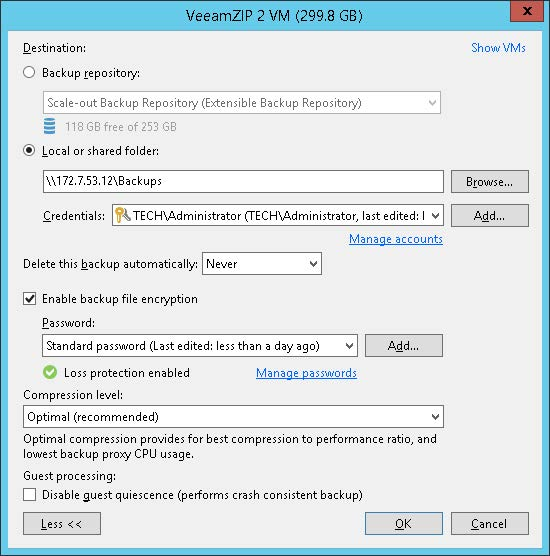
\includegraphics{./images/veeam_zip.jpg}
\caption{Veeam ZIP}\label{Veeam-zip}
\end{figure}

\hypertarget{restore-von-veeamzip}{%
\section{Restore von VeeamZIP}\label{restore-von-veeamzip}}

Um eine VeeamZIP wiederherzustellen muss zunächst oben ``Restore''
geklickt und dann das VeeamZIP-Archiv ausgewählt werden. Anschließend
kann man noch auswählen, wohin die Maschine exportiert werden soll, wie
in Abbildung \ref{Veeam_restore} sehen kann.

\begin{figure}[!htb]
\centering
\includegraphics{./images/veeam_restore.jpg}
\caption{VeeamZIP restore}\label{Veeam-restore}
\end{figure}

\hypertarget{lessons-learned}{%
\section{Lessons Learned}\label{lessons-learned}}

Veeam wird oft als DIE de facto VMware und Hyper-V Backup Lösung
angesehen. Die genialen Aspekte, wie etwa differentielles oder
inkrimentelles Backup sind dabei in der gratis Testversion leider nicht
verfügbar. VeeamZIP hat allerdings gut funktioniert. Zusätzlich
unterstützt Veeam thin und thick Provisioning, was in Praxis Situationen
außerordentliche Flexibilität erlaubt. Außerdem erlaubt Veeams auch in
anderen Hinsichten wahren Enterprise Support. So kann es beispielsweise
mit Copyjobs Backups auf einen externen Speichercluster schreiben. Alles
in allem macht das Veeam genial für Enterprises, für den privaten
Gebrauch scheinen allerdings Backups als ausreichend.
